The Blender software (www.blender.org) was chosen as the simulation environment for our project.
Blender is a free, open source program designed for 3D modeling, physics simulation, and game design. 
Blender provides a means of easily creating 3D objects, attaching properties and constraints to those objects, and developing scripts that interact with the software and objects.

Models in Blender are stored as ``objects'' with associated ``meshes.'' 
A mesh is a data structure with a series of faces, edges, and vertex locations in space for the object. 
Blender also contains methods for adding custom properties to objects, which serves to make the system quite extensible.
Native support for 3D modeling and operations is highly desirable as well. 2D approaches were also considered, but possessed limited support for modeling and manipulating scenes in 3D. 
With Blender's existing 3D support and extensive library utilities for 3D object management, the task of developing a simulation environment is eased considerably.

Blender contains a very accessible Python API. 
This allows Python scripts to access methods in Blender, and allows the system to create and change objects, measure properties of these objects, and even instantiate physical laws (such as gravity) in the scene. 
The direct purpose of this system is to allow Epilog to communicate with a built in series of Python scripts, which then, in turn, will utilize Blender to construct a 3D environment, which can then be examined to derive information about the scene to be fed back as input into Epilog. 
These functions are to be performed incrementally, i.e., in support of a sentence-by-sentence story understanding process. 

The \TDS exists as a series of Python files and a database of objects which interface with Blender. Please note that, from this point on, direct references to structures in the code will be indicated by \texttt{courier} font.

\section{High Level Overview}

The source folder contains three Python files: 
\begin{enumerate}
	\item \texttt{Classes.py}
	\item \texttt{predMethods.py}
	\item \texttt{obutils.py}
\end{enumerate}
A single directory, \texttt{ObjectData}, is also included.

\texttt{Classes.py} file is the highest level Python file, and serves as the top level of the system's organization and control. \texttt{Classes.py} contains three classes: 

\begin{enumerate}
	\item \texttt{Scene} 
	\item \texttt{Entity}
	\item \texttt{Predication} 
\end{enumerate}
	
The \texttt{Scene} class serves to hold the information currently being modeled in the Blender scene, to provide methods for adding entities and predications to the scene, and for querying the scene for how well a given predication is satisfied. 
Although object placement in the system is meant to ensure that all the predications in a given scene are satisfied, this is not necessarily the case. The predications may very well be mutually unsatisfiable, and in keeping with the central purpose of this project, a quick and slightly less accurate placement mechanism is preferable to a more accurate, but much slower one.

Each instantiation of the \texttt{Entity} class stands for an entity in the domain of the scene being modeled. 
An entity is any object in the scene which can be modeled as a Blender mesh object.
The \texttt{Entity} class contains attributes for storing information about the given entity - including a pointer to the object being modeled in the Blender scene - and methods for interacting with the object in the Blender scene.
	
Each instantiation of the \texttt{Predication} class is a predication active in the current scene. 
A \texttt{Predication} instance contains references to the Blender [parent] objects bound by the given predication, and a method for returning placement constraints for either of the objects relative to the other, and one for querying how well the predication is satisfied given the current locations/orientations of the \texttt{Predication}'s objects in the Blender scene. 
The \texttt{Predication} class is generic, and imports placement and querying methods specific to a given predication (e.g. ``near'', ``above'') from the \texttt{Classes.py} file. 

Note that the actual functions for the predication are stored as variables in each class instantiation. 
Once the methods are copied from \texttt{predMethods.py}, \texttt{predMethods.py} is no longer called directly by the predication.

\texttt{predMethods.py} contains placement and query methods for each predicate, for example (respectively) \texttt{nearP} and \texttt{nearQ} for the ``near'' predicate. 
Many of these predicates involve complex functions in Blender's three-dimensional space, which are stored in \texttt{obutily.py}.
\texttt{obutily.py} consists of various methods for operating on Blender objects, and is used by both \texttt{predMethods.py} and \texttt{predMethods.py}.
The full table of the methods for \texttt{predMethods.py} and \texttt{obutils.py} can be viewed in final section.
This ontology was chosen because of how well it fit in with existing Epilog framework. Epilog's internal ontology already defines the domain of discourse into subcategories denoting objects, events, predications, etc. \cite{schubert2000episodic}. Thus, it makes sense to partition the \TDS's ontology similarly. Entities (individuals existing in real space) and predications acting on these entities are explicitly defined in the current model. The other relevant features of the scenes, such as episodes, are built into the framework of the system. For example, an episode is defined as the current arrangement of objects and predications at a given moment within the simulation. This utilizes the built-in model of the \TDS as a specialist is utilized.

\section{Objects and Entities}

The ObjectDatabase directory contains two sub-directories: 

\begin{enumerate}
	\item OBJ 
	\item XML
\end{enumerate}
 
These correspond, respectively, to the two types of information being stored for each object: the three-dimensional model of the object as used by Blender, and other information about the object that is not directly used by Blender. 

In the \TDS, entities are modeled in Blender not with a single mesh, but with separate meshes corresponding to each of the entity's parts. 
When an entity's meshes are imported to the scene, the \texttt{Entity} class imports entity \textless .obj \textgreater-format object files from the \textless item name \textgreater subdirectory in the OBJ directory, where ``item name'' stands for the entity's key (e.g. ``person'' or ``house''). In the Blender scene, these part meshes are bound as children under an empty-point Blender object that is the parent. In the \texttt{Entity} class, the pointer to the Blender object is a pointer to this empty parent object (from which children/parts are easily accessed). Figure \ref{fig:mirs_flow} illustrates the flow of information and interaction between components.

\begin{figure}[h]
	\begin{center}
		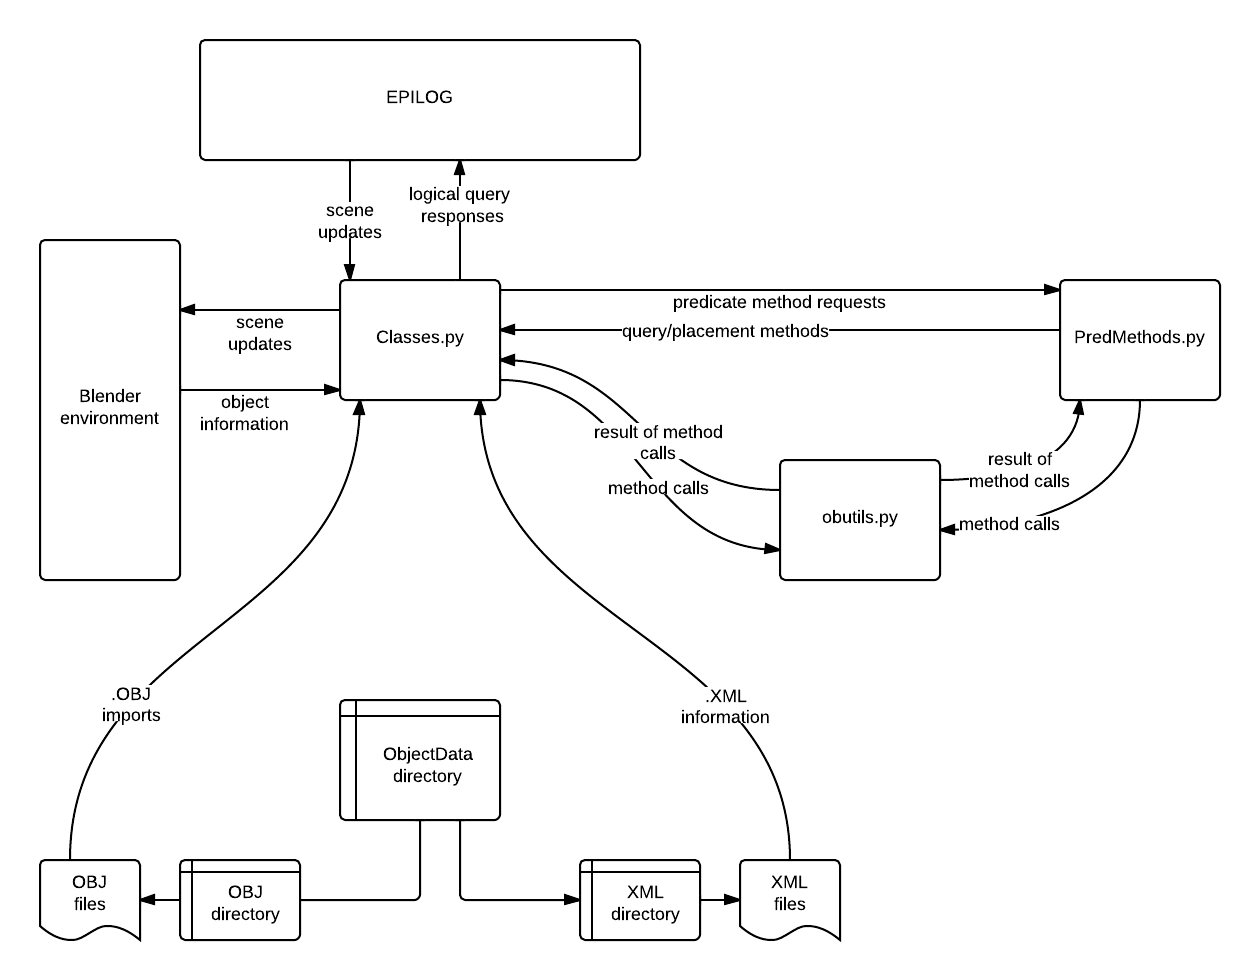
\includegraphics[width=1\textwidth]{figures/mirs_flow.png}
		\caption{The basic flow of information in the \TDS.}
		\label{fig:mirs_flow}
	\end{center}
\end{figure}

The XML directory contains \texttt{\textless item name\textgreater.xml} files for each entity for which there exist Blender models, where \texttt{\textless item name\textgreater} \xspace stands for the entity's key. Each XML file contains the following information: a meronomy graph for the entity, a list of the parts with meshes, and finally bounding box coordinates for the object. 
Periodic updates, predominantly introduction of new objects and predications, as well as changes to existing objects and predications, are sent to the specialist by Epilog.

Although a very extensible sotware system, Blender was not designed specifically for the complex scripting that this project utilized. As such, several object and code issues were encountered with the Blender system that needed to be documented.
First, many of the objects in the system did not have \emph{well-formed} meshes. 
\emph{Well-formed} in this case has very specific meaning. 
In this case, a blender mesh is said to be \emph{well-formed} if it contains closed objects with no holes in the mesh, edge loops (which define faces) which are connected and form a closed loop, and no disconnected components. 
Unfortunately, several objects in the system (notably the “chair” object) contain some glitch in their meshes which renders them not \emph{well-formed}. 
This can cause several errors when intersection and difference algorithms (or other methods which involve mesh operations) are utilized by the system.
These changes were made, and the objects were able to function correctly.

There are further limiting factors that were noted when utilizing Blender to place and measure objects. Due to the algorithms used in the volume calculation:

\begin{center}
	\begin{itemize}
		\item Faces and Edges cannot be placed directly on top of one another, an offset (even as small as 0.001 BU) of one of the objects must be used
		\item Even if an object is deleted from Blender's scene environment, it's mesh information will still remain. This can slow down the computation of built-in functions in blender whose run-time scales with the total number of meshes in the scene. As such, scenes must be restarted for multiple rounds of testing to ensure accurate, releiable data.
	\end{itemize}
\end{center}

\section{Predications}
My particular work has focused on the construction of the predicate class, as well as the helper methods in \texttt{obutily.py}, and management and organization of the program files.
Each \texttt{Predication} instance contains two methods: \texttt{Place()} and \texttt{Query()}. These predicates are stored as \texttt{\textless predicate name\textgreater P} and \texttt{\textless predicate name\textgreater Q}. 
As shown above, the placement function of the near predication is \texttt{nearP} and the query function is \texttt{nearQ}. Query methods evaluate the scene and return a value for how well the given predicate is satisfied in the current scene. 
This can be done continuously as a value between 0.0 and 1.0, or as a boolean. 
For a boolean value, the continuous answer is still evaluated: 1.0 is returned if the answer is above 0.5, and 0.0 if below.
The purpose of the \texttt{BinaryFlag} attribute in the \texttt{Predication} class is to determine whether the predicate is evaluated as a boolean value or not.



\subsection{Vision Predication}
By far, the largest and most complicated predicate was \texttt{canSee(A,B)}.
The implementation of this function relied heavily on ray-casting and went through several iterations before a sufficient model and algorithm were developed. 
The querying method for this predication originally was to be implemented as a single ray-cast, from one object's center to another.

A number of different attempts to construct a sufficient \texttt{canSee(A,B)} function were tested, yet none were of the quality needed for the project. Examples include the use of a conical object expanding from entity A's ``eye'' to B and noting the percent of B's volume that was encompassed inside. Several functions in Blender's Game Engine were also implemented. Early on, a function existed which ray-casted from the center-point of A to the center point of B. This function was naively simple, but proved itself to be surprisingly difficult to implement. For a graphical representation, Figure \ref{fig:vision1} below illustrates the ideal for this model. Note that in this (and future) diagrams, a solid line represents the actual ray cast, and a dotted line represents the remainder distance that the cast would have traveled if there had not been an object in the way acting as an interrupting agent.	
	
\begin{figure}[h]
	\begin{center}
		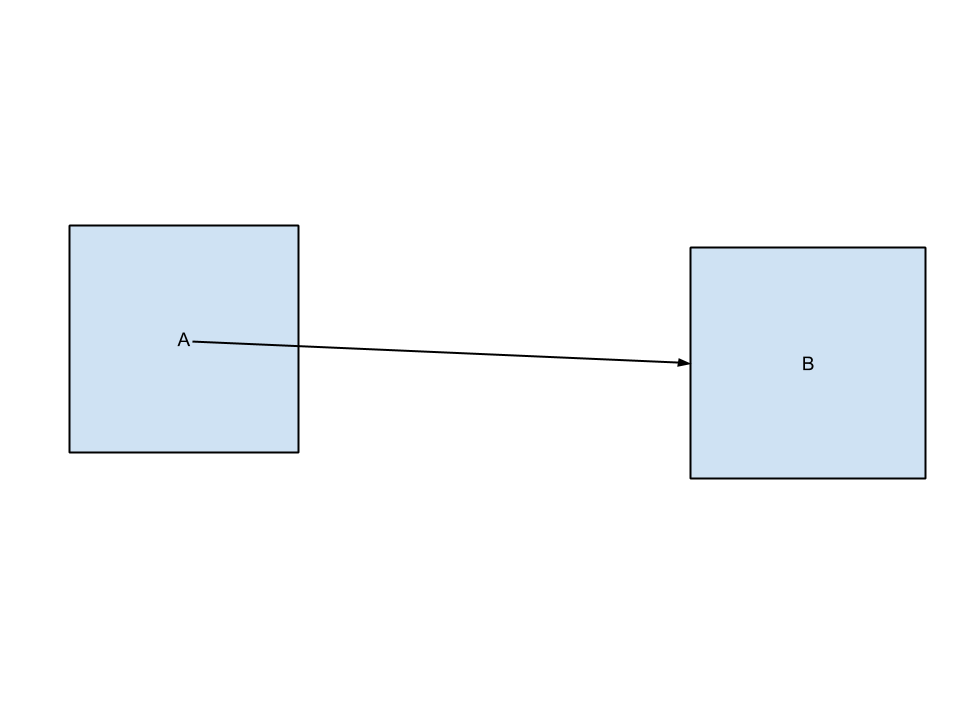
\includegraphics[width=0.48\textwidth]{figures/vision1.png}
	\end{center}
	\caption{an idealized model of the naive implementation of \texttt{canSee(A,B)}.}
	\label{fig:vision1}
\end{figure}

One issue that came up with this design was the collision nature of ray-casting. Namely, a given ray-cast in Blender will return when it hits an object, any object. This means that casts from A's center would always stop upon hitting A's outer mesh. One early attempt to solve this was to simply implement repeated casting: the method would cast continuous rays from the end of one to the start of the other until the end object was met. Figure \ref{fig:vision2} shows the idealized version of the function of this implementation of the function.

\begin{figure}[h]
	\begin{center}
		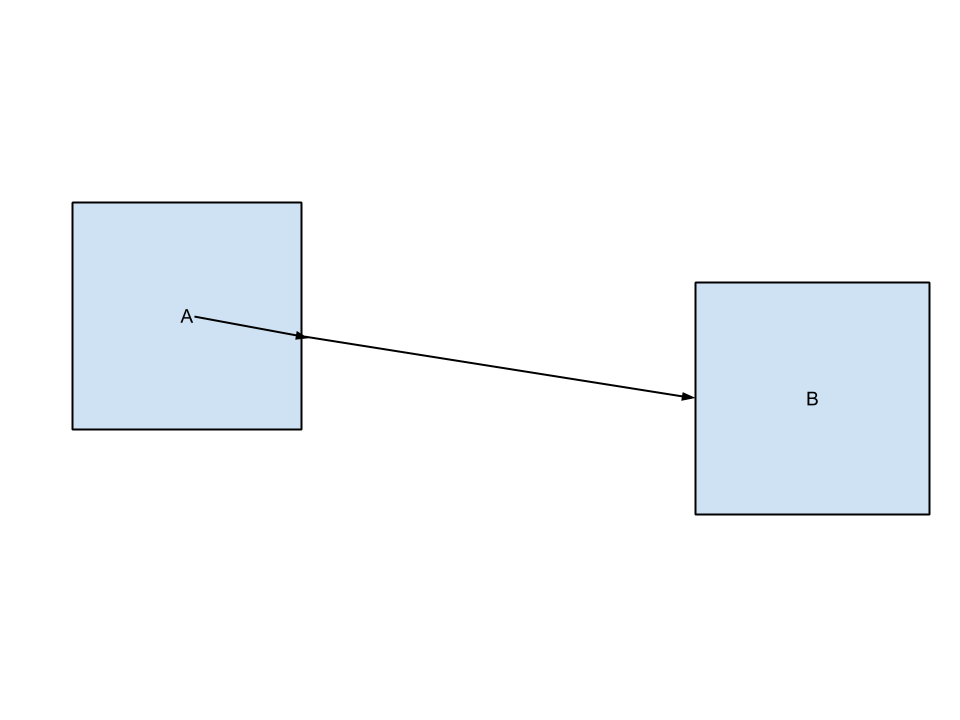
\includegraphics[width=0.48\textwidth]{figures/vision2.png}
	\end{center}
	\caption{A second implementation of ray-casting}
	\label{fig:vision2}
\end{figure}

This revealed yet another problem, however, as casting from the face of one object (which was the collision point of the fist ray-cast in the above) would simply return the starting point of the cast. The ray-cast could repeat infinite times and still be stuck on the same point. The third iteration of this function was meant to fix this. This iteration involved the addition of another method in \texttt{obutily.py}, \texttt{nudge}, which would return an infinitesimally small distance closer to the end point. This function allowed repeated ray-casting to continue unabated and as planned. The new model for ray-casting in this simple iteration is illustrated in figure \ref{fig:vision3}. 

\begin{figure}[h]
	\begin{center}
		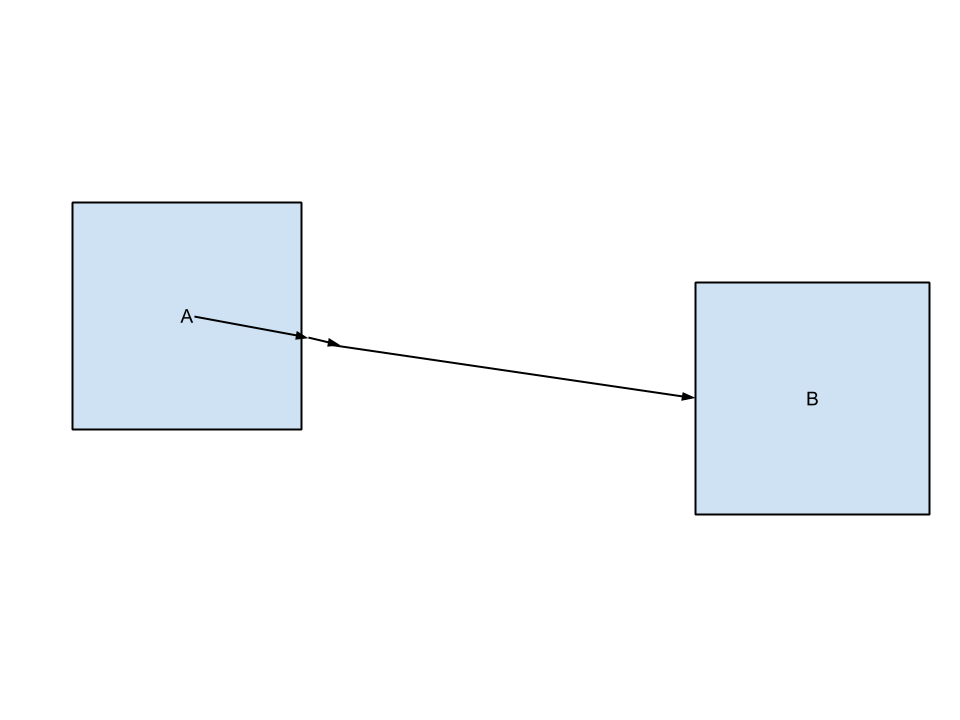
\includegraphics[width=0.48\textwidth]{figures/vision3.png}
	\end{center}
	\caption{The nudge addition to the naive model}
	\label{fig:vision3}
\end{figure}

This model was able to accurately cast a ray from the center of A to B, stopping when it hit B's outer mesh. However, the naive model was, as the name should suggest, not sufficient and could easily return erroneous answers. For example, if there was an object in between A and B which could block the cast, then the method would conclude that A could not see B, even if it were obvious that a line of sight existed between the two. Figure \ref{fig:vision4} illustrates this.

\begin{figure}[h]
	\begin{center}
		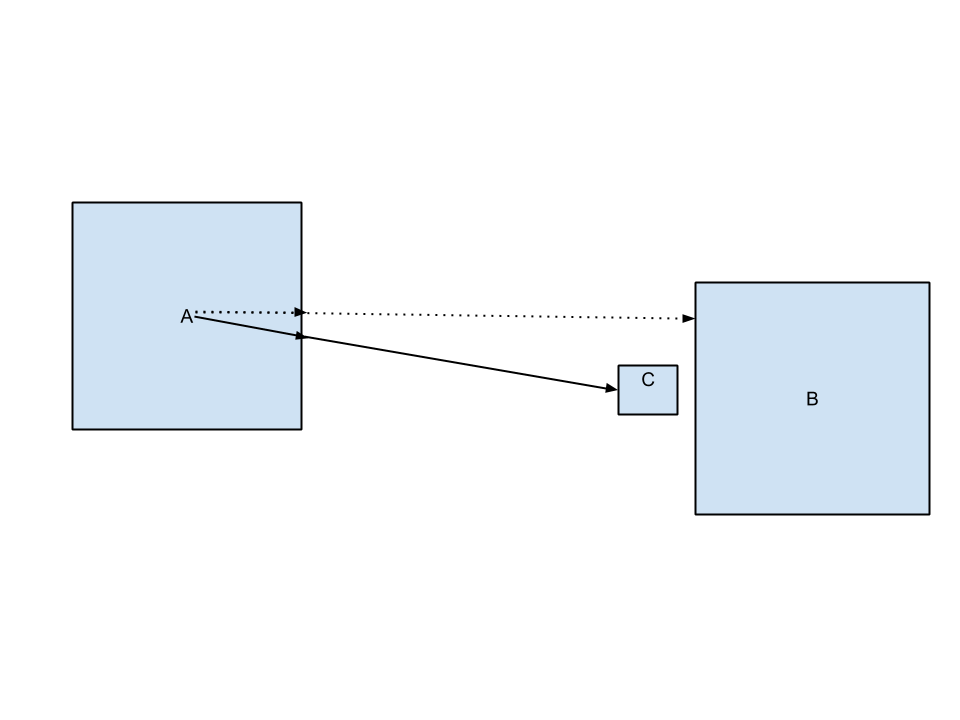
\includegraphics[width=0.48\textwidth]{figures/vision4.png}
	\end{center}
	\caption{C blocks the site of A, even though there exist obvious casts (dashed) that would indicate that B is visible}
	\label{fig:vision4}
\end{figure}

It was obvious early on that this implementation would only serve as a template for future endeavors.
The second model cast a slew of rays from A to the vertices of B. This improved over the naive implementation in two ways. First, it allowed a varying degrees of visibility. Several of the rays may reach their target, and several may not, which allowed for a sense of “partial obscurity” which was not allowed in the original model. This ran into a small technical issue early on, however, as rays would not return if they made contact with the vertices of an object. Due to a technicality in Blender, casts would only return if they made contact with the face of an object. As such, a modification of the nudge function was implemented which pushed the end point of the casts closer to the center. This way, there was a guarantee that the casts, if unobstructed, would hit the object properly. Figure \ref{fig:vision5} illustrates this model.

\begin{figure}[h]
	\begin{center}
		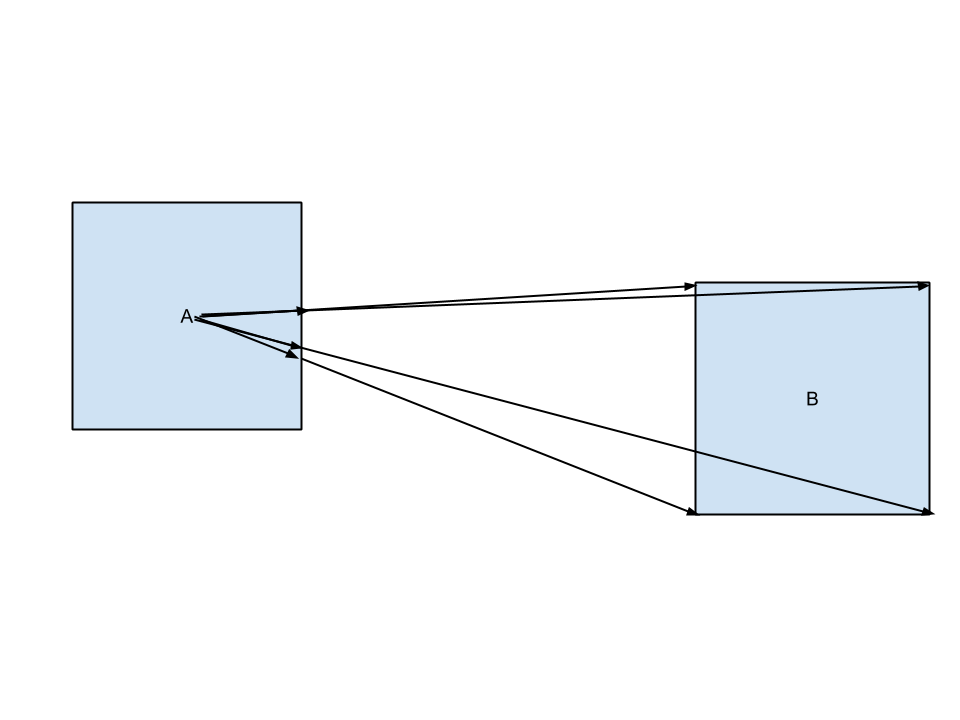
\includegraphics[width=0.48\textwidth]{figures/vision5.png}
	\end{center}
	\caption{The second iteration of the \texttt{canSee(A,B)} algorithm}
	\label{fig:vision5}
\end{figure}

This model was not perfect, however, in that it could give bias to a section of an object if there were a large number of vertices concentrated at a given section. In figure \ref{fig:vision6}, we show how this could be problematic. In this example, A would cast a disproportionate amount of rays to B's bottom side, which would collide with C, giving the impression that B is much less visible than it actually is.

\begin{figure}[h]
	\begin{center}
		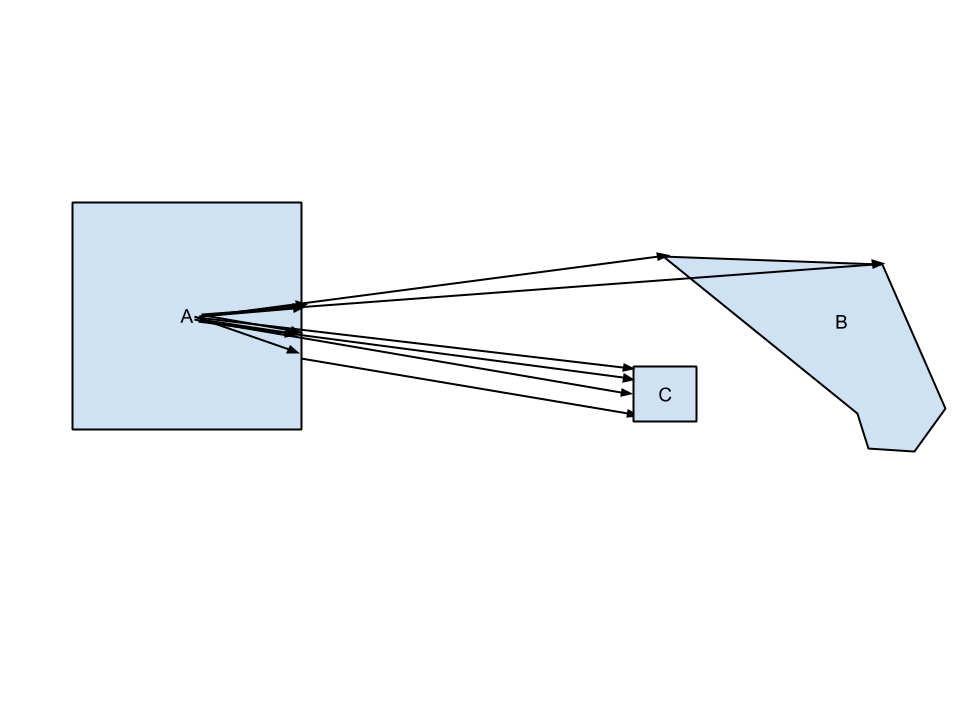
\includegraphics[width=0.48\textwidth]{figures/vision6.png}
	\end{center}
	\caption{The majority of the casts are blocked by C even though B is visible.}
	\label{fig:vision6}
\end{figure}

One suggested solution to this situation involved weighting the vertices depending on how close they were. In this interpretation, casts to close-by vertices would be “worth less.” If these successfully hit their target, they would return a number less than one. The exact weighting system was not decided. This system, however, proved to be unnecessary, as the final algorithm removed the need for vertices entirely. 

The final system utilized an obscure library in Blender Python (\texttt{BPY\_extras}) to grasp random points on the meshes faces. Rays were cast to these points, and the percent of casts that returned were used to evaluate the visibility of the target object. This method was both fair and correct. The number of rays cast to a given face was proportional to the face's percent of the total surface area of the object, which ensured that the most visible (largest) faces would receive the most casts. Because the number of samples is proportional to the size of the object's faces, no section of the object will over represent itself in testing. Figure \ref{fig:vision7} shows how the new method solves the problems of the old.

\begin{figure}[h]
	\begin{center}
		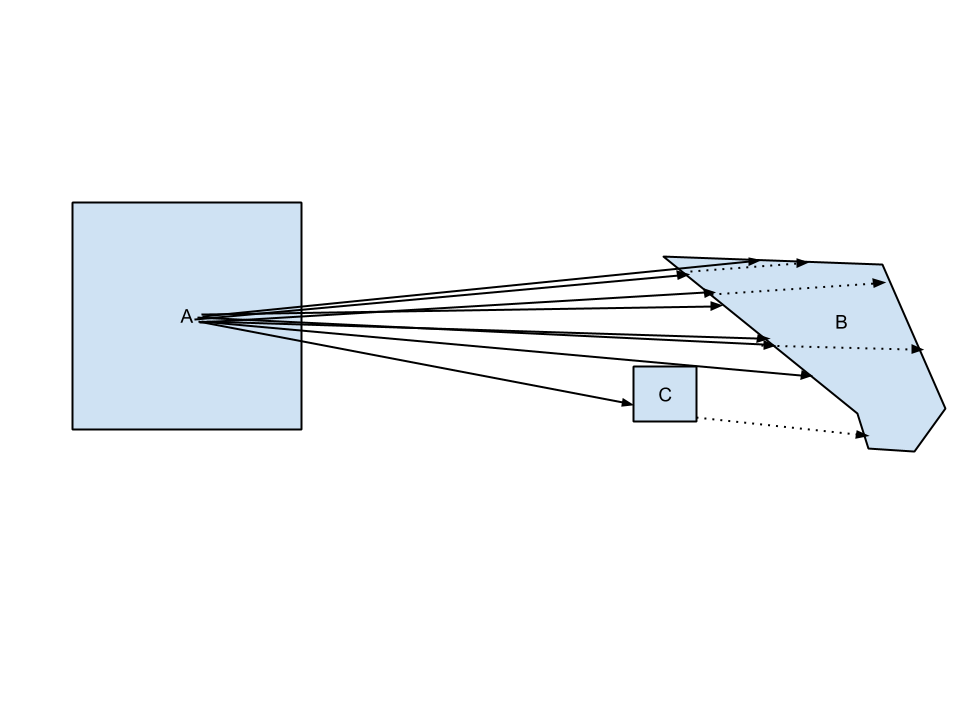
\includegraphics[width=0.48\textwidth]{figures/vision7.png}
	\end{center}
	\caption{Rays are cast evenly across object B.}
	\label{fig:vision7}
\end{figure}

The final change to the vision predication involved compensation for opacity. It was desired that the visibility of an entity not simply depend on line of sight, but also on the presence of partially occluding objects passed through en route to the goal object. This was solved through custom properties and repeated casting. Each ray-cast was given an initial value of 1. The cast traveled through space as in the above model. When another object was encountered, the behavior of the cast differed depending on the object hit. If the object was the target object, then the cast returned it's value (initially set to one). If it encountered a different object with no occlusion property (or an occlusion value of one) then the hit object was assumed to be completely opaque and the cast returned zero. A completely opaque object (one that would cause any ray to return 0 if it made contact), was specified with an occlusion of -1. If the object hit an object with an occlusion value between zero and one, then the object recast towards its target, but the value of the occlusion property was added to an “occlusion counter” for the cast. This occlusion counter would would be reduced by the occlusion amount of the object when the cast left the object.	

As the cast traveled through an object, the value would degrade proportional to the current counter. If the return value was reduced to zero, then the cast would fail and the function would return zero. Thus, the further through an obscuring object (such as a fog or the leaves of a tree) an object was, the more obscured it became. The “occlusion counter” was necessary in order to allow multiple obscuring factors affect the object. This corresponds to situations such as man looking at a bird through a tree in a fog.

The addition of occlusion necessitated the introduction of a new function in \texttt{obutily.py}: \texttt{cast\_thru}. This function performed all of the above functions, and took care of the repeated casting (including calls to ray\_cast and nudge). The initial cast was handled by the \texttt{predicateMethods.py} file, and subsequent casts were all done in the \texttt{cast\_thru method}. This led \texttt{canSee} to a slightly different larger dependence on \texttt{obutily.py} functions than other predications.


Originally, the starting point for \texttt{canSee} was the location of the first object in the predication.
Typically, this was the lowest point in the object, in the center of the xy plane. 
This presents an obvious issue for calculating visibility: human beings do not see with their feet. 
Thus, for models which were capable of vision, an additional ``eye'' was added to list of meshes. 
The \texttt{canSee} function was changed to begin ray tracing from the location of the eye, which was located just in front of the face of the figures. 

\subsection{Placement Methods}

\texttt{Place()} returns the areas in the Blender scene where the predicate holds for one entity relative to the other. This makes the assumption that the second object has already been placed; for example in the predication ``near(A,B)'', if \texttt{Place(A)} was called, it would return an acceptance area of ``nearness'' for A, such that the predication is satisfied. 
At present, the placement locations are returned as a tuple of pairs, with each pair containing the minimum and maximum values for the x, y, and z dimensions. This was meant to build of previous (similar) methods in Wordseye and Soar, which used similar methodology. \cite{wordseye,wintermute2009overview}.
The placement functions went through several iterations and different ideas, and were the subject of much revision over the course of the project.
For the first build of the project, the current system was implemented. Figure \ref{fig:square_placement} provides a visualization for this method.
 
\begin{figure}[h]
	\begin{center}
		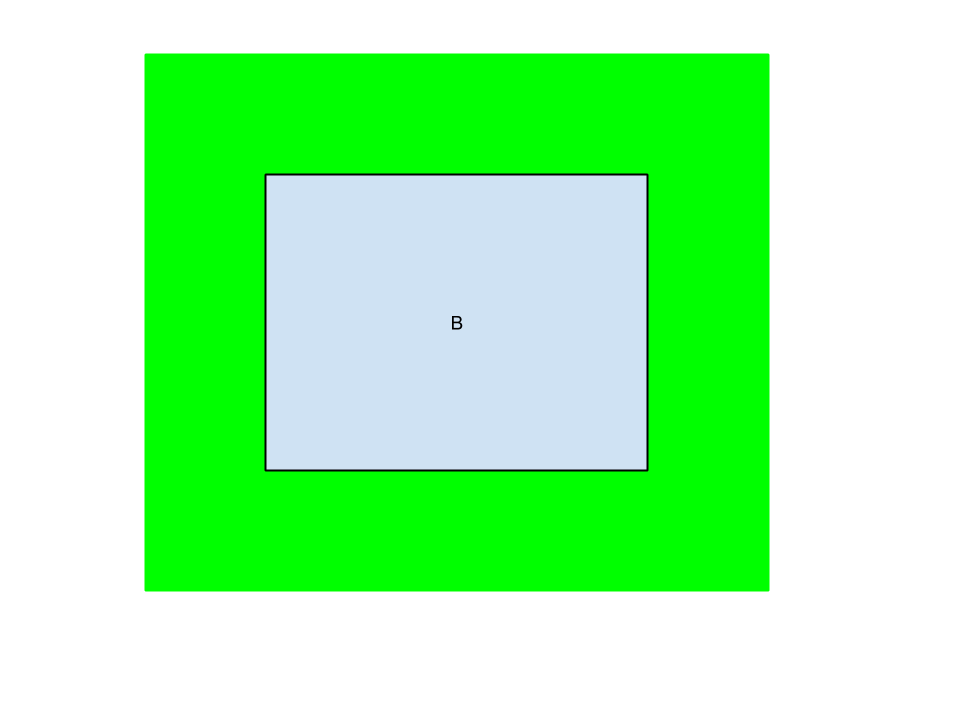
\includegraphics[width=0.48\textwidth]{figures/square_placement.png}
	\vspace{-1cm}
	\caption{A visualization of the first and current placement mechanism.}
	\label{fig:square_placement}
	\end{center}
\end{figure}

This system suffices for many predicates; however, it is not easily extensible to predications which have disjoint or disconnected valid placement areas. 
As such, there were concerns about whether a better placement paradigm was necessary.
In particular, the vision predicates can generate placement areas of this sort. Figure \ref{fig:vision_placement_theoretical} illustrates the issues that the system raised.

\begin{figure}[h]
	\begin{center}
		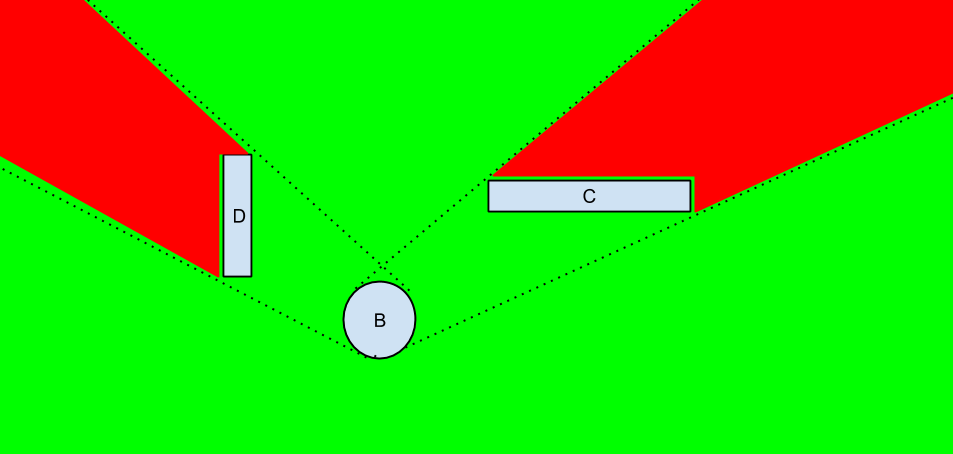
\includegraphics[width=0.48\textwidth]{figures/vision_placement_theoretical.png}
	\caption{The theoretical placement areas for the predicate \texttt{canSee}. Valid areas are colored green, invalid areas are red.}
	\label{fig:vision_placement_theoretical}
	\end{center}
\end{figure}

Several solution have been researched and proposed. Wordseye utilizes a the concept of ``valid placement polygons.'' 
This concept represents the valid placement areas of objects as polygons, and, with this heuristic, is able to choose the best area for inserting an object in a scene \cite{wordseye}. 
Another similar solution is proposed in Xu et al, where Minkowsky sums are utilized. This technique has been shown to be efficient in certain special cases of polygons, and was able to produce fruitful results in experimental trials \cite{xu2002constraint}. 

In this vein, I proposed the idea of utilizing multiple of our current placement rectangular-prisms (and their combinations) in order to represent the valid placement areas of a given polygon. 
This idea has been worked on and refined this idea into several possible solutions. One solution is the idea of the ``grid-box technique.'' 
In this technique, the geometry of placement areas is represented as an assembly of discrete 'boxes', one of which is sampled for a valid placement location of the given object.
Each box is represented a 3-tuple of pairs, corresponding to x, y, and z coordinates of a cube in three-dimensional space. 
These boxes, unlike their counterparts in the current placement system, are of a discrete and unchanging size, and are arranged in a tessellating fashion similar to a grid. 
In this method, a square is considered a valid placement area if all of it's points satisfy a the respective predication. Figure \ref{fig:grid_placement} below provides an illustration.

\begin{figure}[h]
	\begin{center}
		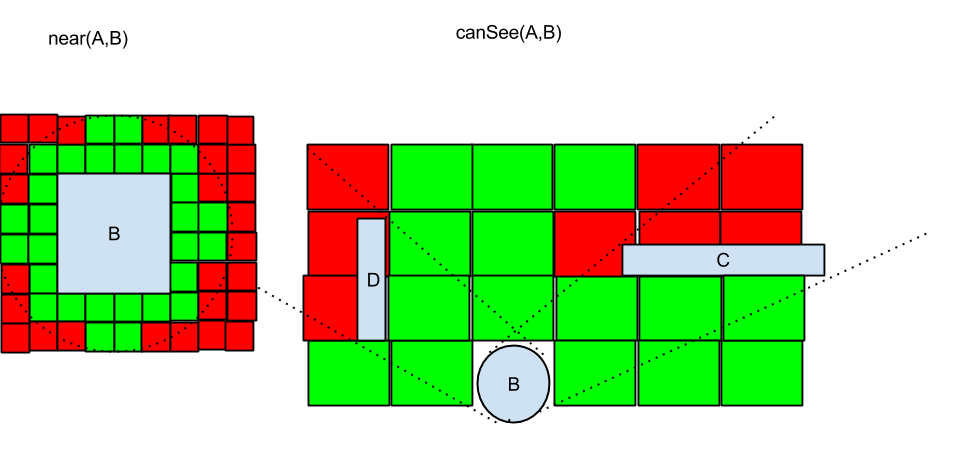
\includegraphics[width=0.48\textwidth]{figures/grid_placement.png}
	\caption{One proposed method of placing objects using by using a uniform grid of placement areas.}
	\label{fig:grid_placement}
	\end{center}
\end{figure}

Another proposed method is the rejection-sampling model. 
A short mockup of it was even built earlier this year. 
This model randomly selects points given a heuristic for the model, and rejects them if they fails to satisfy the specified predication or predications. 
\ref{fig:rejection_sampling_placement} below illustrates the system.

As previously noted, this system does allow for a very simple implementation (forgoing the placement prism entirely), though because it rejects so many potential points, The feasibility of this algorithm was a subject of investigation. 

A combination of rejection sampling and the standard ``block placement'' algorithm was used. The collective blocks of all the predications of an object are overlayed, their intersection being the new legal placement area. Rejection sampling is then used to sample locations from this space. The resulting configuration is queried. If all the predications are satisfied, the next object is placed. If it is not, then another spot is sampled, and the process begins again.

\begin{figure}[h]
	\begin{center}
		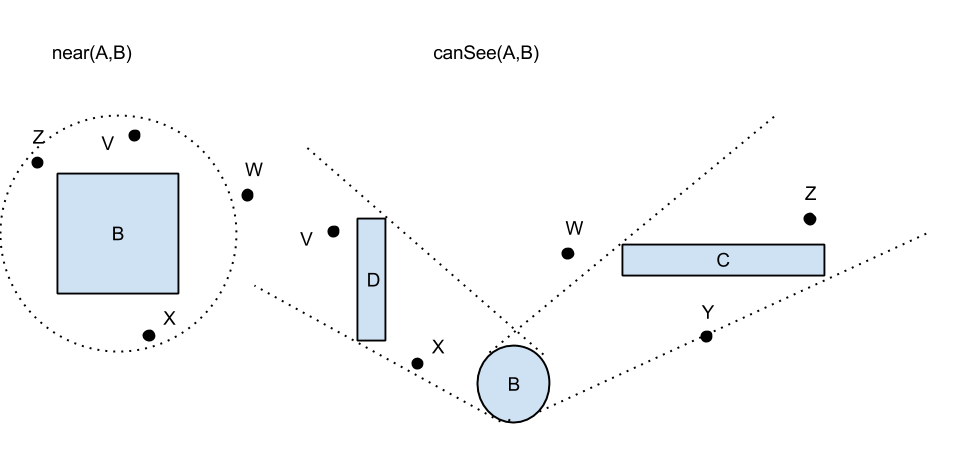
\includegraphics[width=0.48\textwidth]{figures/rejection_sampling_placement.png}
	\caption{Rejection sampling was also considered as a placement mechanism.}
	\label{fig:rejection_sampling_placement}
	\end{center}
\end{figure}